%%%%%%%%%%%%%%%%%%%%%%%%%5
%% abtex2-modelo-trabalho-academico.tex, v<VERSION> laurocesar
%% Copyright 2012-<COPYRIGHT_YEAR> by abnTeX2 group at http://www.abntex.net.br/
%%
%% This work may be distributed and/or modified under the
%% conditions of the LaTeX Project Public License, either version 1.3
%% of this license or (at your option) any later version.
%% The latest version of this license is in
%%   http://www.latex-project.org/lppl.txt
%% and version 1.3 or later is part of all distributions of LaTeX
%% version 2005/12/01 or later.
%%
%% This work has the LPPL maintenance status `maintained'.
%%
%% The Current Maintainer of this work is the abnTeX2 team, led
%% by Lauro César Araujo. Further information are available on
%% http://www.abntex.net.br/
%%
%% This work consists of the files abntex2-modelo-trabalho-academico.tex,
%% abntex2-modelo-include-comandos and abntex2-modelo-references.bib
%%

% ------------------------------------------------------------------------
% ------------------------------------------------------------------------
% abnTeX2: Modelo de Trabalho Academico (tese de doutorado, dissertacao de
% mestrado e trabalhos monograficos em geral) em conformidade com
% ABNT NBR 14724:2011: Informacao e documentacao - Trabalhos academicos -
% Apresentacao
% ------------------------------------------------------------------------
% ------------------------------------------------------------------------

\documentclass[
	% -- opções da classe memoir --
	12pt,				% tamanho da fonte
%  openright,			% capítulos começam em pág ímpar (insere página vazia caso preciso)
	oneside,			% para impressão em recto e verso use twoside
	a4paper,			% tamanho do papel.
	% -- opções da classe abntex2 --
	%chapter=TITLE,		% títulos de capítulos convertidos em letras maiúsculas
	%section=TITLE,		% títulos de seções convertidos em letras maiúsculas
	%subsection=TITLE,	% títulos de subseções convertidos em letras maiúsculas
	%subsubsection=TITLE,% títulos de subsubseções convertidos em letras maiúsculas
	% -- opções do pacote babel --
	english,			% idioma adicional para hifenização
	french,				% idioma adicional para hifenização
	spanish,			% idioma adicional para hifenização
	brazil				% o último idioma é o principal do documento
	]{abntex2}

% ---
% Pacotes básicos
% ---
\usepackage{times}			    % Usa fonte times
\renewcommand{\ABNTEXchapterfont}{\normalfont} % para aplicar a fonte escolhida em tudo
\usepackage[T1]{fontenc}		% Selecao de codigos de fonte.
\usepackage[utf8]{inputenc}		% Codificacao do documento (conversão automática dos acentos)
\usepackage{lastpage}			% Usado pela Ficha catalográfica
\usepackage{indentfirst}		% Indenta o primeiro parágrafo de cada seção.
\usepackage{color}				% Controle das cores
\usepackage{graphicx}			% Inclusão de gráficos
\usepackage{microtype} 			% para melhorias de justificação
% ---

% ---
% Pacotes adicionais, usados apenas no âmbito do Modelo Canônico do abnteX2
% ---
\usepackage{lipsum}				% para geração de dummy text
% ---

% ---
% Pacotes de citações
% ---
\usepackage[brazilian,hyperpageref]{backref}	 % Paginas com as citações na bibl
\usepackage[alf]{abntex2cite}	% Citações padrão ABNT

% ---
% CONFIGURAÇÕES DE PACOTES
% ---

% ---
% Configurações do pacote backref
% Usado sem a opção hyperpageref de backref
\renewcommand{\backrefpagesname}{Citado na(s) página(s):~}
% Texto padrão antes do número das páginas
\renewcommand{\backref}{}
% Define os textos da citação
\renewcommand*{\backrefalt}[4]{
	\ifcase #1 %
		Nenhuma citação no texto.%
	\or
		Citado na página #2.%
	\else
		Citado #1 vezes nas páginas #2.%
	\fi}%
% ---

% ---
% Informações de dados para CAPA e FOLHA DE ROSTO
% ---
\titulo{Título do trabalho}
\autor{Nome do autor}
\data{2019}
\local{Cidade - UF}
\orientador{Nome-do-Orientador}
\coorientador{}
\instituicao{%
  Universidade/Faculdade do Brasil
  \par
  Meu-curso
}
\tipotrabalho{Monografia}

% O preambulo deve conter o tipo do trabalho, o objetivo (propósito),
% o nome da instituição e a área de concentração.
% Esse texto irá compor a Folha de Rosto e Folha de Aprovação.
\preambulo{
O empenho em analisar a revolução dos costumes exige a precisão e a
definição dos procedimentos normalmente adotados.
\newline\textbf{Área de concentração}: Computação.
}%% fim do preambulo




% ---
% Configurações de aparência do PDF final

% alterando o aspecto da cor azul
\definecolor{blue}{RGB}{41,5,195}

% informações do PDF
\makeatletter
\hypersetup{
     	%pagebackref=true,
		pdftitle={\@title},
		pdfauthor={\@author},
    	pdfsubject={\imprimirpreambulo},
	    pdfcreator={LaTeX with abnTeX2 and Limarka},
		pdfkeywords={abnt}{latex}{abntex}{abntex2}{trabalho acadêmico}{limarka},
		colorlinks=false,       		% false: boxed links; true: colored links
    	linkcolor=black,          	% color of internal links
    	citecolor=black,        		% color of links to bibliography
    	filecolor=black,      		% color of file links
		urlcolor=black,
		bookmarksdepth=4
}
\makeatother
% ---

% ---
% Possibilita criação de Quadros e Lista de quadros.
% Ver https://github.com/abntex/abntex2/issues/176
%
\newcommand{\quadroname}{Quadro}
\newcommand{\listofquadrosname}{Lista de quadros}

\newfloat[chapter]{quadro}{loq}{\quadroname}
\newlistof{listofquadros}{loq}{\listofquadrosname}
\newlistentry{quadro}{loq}{0}

% configurações para atender às regras da ABNT
\setfloatadjustment{quadro}{\centering}
\counterwithout{quadro}{chapter}
\renewcommand{\cftquadroname}{\quadroname\space}
\renewcommand*{\cftquadroaftersnum}{\hfill--\hfill}

% ---


% ---
% Espaçamentos entre linhas e parágrafos
% ---

% O tamanho do parágrafo é dado por:
\setlength{\parindent}{1.3cm}

% Controle do espaçamento entre um parágrafo e outro:
\setlength{\parskip}{0.2cm}  % tente também \onelineskip

% ---
% compila o indice
% ---
\makeindex
% ---

%---
% CONFIGURAÇÕES EXTRA DO LIMARKA
%---

% Configura citações de pandoc para 4cm à esquerda (utiliza o ambiente quote)
\renewenvironment{quote}
  {\small\list{}{\rightmargin=0.1cm \leftmargin=4cm}%
   \item\relax}
  {\endlist}

% Para incluir páginas PDF (ficha catalografica e folha de aprovação)
\usepackage[dvipsnames]{xcolor} % http://tex.stackexchange.com/questions/124636/package-xcolor-error-undefined-colors-maroon-royal-blue-when-master-has-pdf
\usepackage{pdfpages}
\usepackage{longtable,ltcaption,booktabs} % para as tabelas pandoc e quadros ABNT
%\usepackage{floatrow}
%\floatsetup[figure]{capposition=top}

% Para melhorar o visual do quadro
\usepackage{boldline} 
\def\toprule{\hlineB{3}} % primeira linha mais gorda
\def\midrule{\hline}
\def\bottomrule{\hlineB{3}} % última linha mais gorda



% ---
% BUG: Imagens e tabelas apareciam no meio da página em branco
% https://github.com/abntex/trabalho-academico-limarka/issues/1
% O código a seguir posta imagens ou tabelas em página em branco no topo, em vez do meio (comportamento padrão)
\makeatletter
\setlength{\@fptop}{5pt} % Set distance from top of page to first float
\makeatother
% ---

% ---
% Usado pelo limarka como hook para criação de novas listas.
% https://github.com/abntex/trabalho-academico-limarka/issues/16
%
\newcommand{\listasdousuario}{}

% ---
% CUSTOMIZAÇÕES DO USUÁRIO (somente se existir arquivo config/latexcustomizacao.sty)
% ---
\IfFileExists{latexcustomizacao.sty}{\usepackage{latexcustomizacao}}{}

%%
%% Esse modelo é responsável pela impressão dos seguintes elementos:
%% Capa, Folha de rosto e Ficha catalográfica.

\special{dvipdfmx:config z 0}

% ----
% Início do documento
% ----
\begin{document}

% Seleciona o idioma do documento (conforme pacotes do babel)
%\selectlanguage{english}
\selectlanguage{brazil}

% Retira espaço extra obsoleto entre as frases.
\frenchspacing

% ----------------------------------------------------------
% ELEMENTOS PRÉ-TEXTUAIS
% ----------------------------------------------------------
% \pretextual

% ---
% Capa 
% ---
% Gerando capa abnTeX2
\imprimircapa

% ---

% ----------------------------------------------------------
% ELEMENTOS PRÉ-TEXTUAIS
% ----------------------------------------------------------
% \pretextual

% ---
% Folha de rosto: sempre será impressa
% ---
\imprimirfolhaderosto

% ---
% Sem ficha catalográfica
% ---
% ---


% ---
% ERRATA: Sem errata
% ---


% ---
% Sem Folha de aprovação
% ---
% ---
% ---
% Dedicatória
% ---
\begin{dedicatoria}
   \vspace*{\fill}
   \centering
   \noindent

    Cacilds vidis litro abertis. Em pé sem cair, deitado sem dormir, sentado
    sem cochilar e fazendo pose. Morbi viverra placerat justo, vel pharetra
    turpis. Interagi no mé, cursus quis, vehicula ac nisi. Ô gente finis,
    pode baixar uma ampolis que hoje é sexta-feris!

   \vspace*{\fill}
\end{dedicatoria}
% ---
% ---
% Agradecimentos
% ---
\begin{agradecimentos}

No entanto, não podemos esquecer que o aumento do diálogo entre os
diferentes setores produtivos promove a alavancagem das posturas dos
órgãos dirigentes com relação às suas atribuições.

\end{agradecimentos}
% ---
% ---
% Epígrafe
% ---
% ---

% ---
% Resumo na língua vernácula (obrigatório)
% ---


% resumo em português
\setlength{\absparsep}{18pt} % ajusta o espaçamento dos parágrafos do resumo
\begin{resumo}

  A nível organizacional, o entendimento das metas propostas representa
  uma abertura para a melhoria das condições financeiras e administrativas
  exigidas.

 \textbf{Palavras-chave}: Markup Language, Markdown, Normas da ABNT, Latex, Limarka
\end{resumo}


% ---
% Resumo em língua estrangeira (obrigatório)
% ---

% resumo em inglês
\begin{resumo}[Abstract]
 \begin{otherlanguage*}{english}
   Todavia, o aumento do diálogo entre os diferentes setores produtivos
   apresenta tendências no sentido de aprovar a manutenção das condições
   financeiras e administrativas exigidas.

   \vspace{\onelineskip}
 
   \noindent 
   \textbf{Keywords}: 
 \end{otherlanguage*}
\end{resumo}

% resumo em francês 
\begin{resumo}[Résumé]
 \begin{otherlanguage*}{french}
    At the organizational level, understanding the proposed goals represents
    an opening for the improvement of the required financial and
    administrative conditions.
 
   \textbf{Mots-clés}: 
 \end{otherlanguage*}
\end{resumo}

% resumo em espanhol
\begin{resumo}[Resumen]
 \begin{otherlanguage*}{spanish}
   A nivel organizacional, la comprensión de las metas propuestas
   representa una apertura para la mejora de las condiciones financieras y
   administrativas requeridas.
  
   \textbf{Palabras clave}: 
 \end{otherlanguage*}
\end{resumo}
% ---

% ---
% Lista de ilustrações (opcional): não utilizando.
% ---


% ---
% Lista de quadros (opcional): não utilizando.
% ---

% Carrega listas definidas pelo usuário em `latexcustomizacao.sty`
\listasdousuario
% ---
% Lista de tabelas (opcional): não utilizando
% ---

% ---
% Lista de abreviaturas e siglas (opcional)
% ---
\begin{siglas}
  \item[ABNT] Associação Brasileira de Normas Técnicas
\end{siglas}
% ---

% ---
% Lista de símbolos (opcional): AUSENTE
% ---
% ---
% Sumário
% ---
\pdfbookmark[0]{\contentsname}{toc}
\tableofcontents*
\cleardoublepage
% ---


% ----------------------------------------------------------
% ELEMENTOS TEXTUAIS
% ----------------------------------------------------------
\textual
\pagestyle{simple}                  % #17 Cabeçalho apenas com
\aliaspagestyle{chapter}{simple}    % a numeração das páginas


\hypertarget{introduuxe7uxe3o}{%
\chapter{Introdução}\label{introduuxe7uxe3o}}

A prática cotidiana prova que o aumento do diálogo entre os diferentes
setores produtivos obstaculiza a apreciação da importância de
alternativas às soluções ortodoxas. O cuidado em identificar pontos
críticos no comprometimento entre as equipes causa impacto indireto na
reavaliação do levantamento das variáveis envolvidas.

É claro que a execução dos pontos do programa obstaculiza a apreciação
da importância do impacto na agilidade decisória. Gostaria de enfatizar
que a percepção das dificuldades possibilita uma melhor visão global das
diversas correntes de pensamento. É claro que a expansão dos mercados
mundiais é uma das consequências do fluxo de informações.

É importante questionar o quanto a hegemonia do ambiente político
representa uma abertura para a melhoria da gestão inovadora da qual
fazemos parte. Todavia, a valorização de fatores subjetivos garante a
contribuição de um grupo importante na determinação do fluxo de
informações.

Gostaria de enfatizar que a complexidade dos estudos efetuados
obstaculiza a apreciação da importância das posturas dos órgãos
dirigentes com relação às suas atribuições.

\hypertarget{motivauxe7uxe3o}{%
\section{Motivação}\label{motivauxe7uxe3o}}

A escolha do tema para este TCC não foi um acaso, mas o resultado de uma
jornada de descobertas, paixões e questionamentos que marcaram
profundamente minha trajetória acadêmica.

\hypertarget{objetivos}{%
\section{Objetivos}\label{objetivos}}

\hypertarget{objetivo-geral}{%
\subsection{Objetivo geral}\label{objetivo-geral}}

Apresentação do objetivo geral.

\hypertarget{objetivos-especuxedficos}{%
\subsection{Objetivos específicos}\label{objetivos-especuxedficos}}

\begin{itemize}
\tightlist
\item
  objetivo 1;
\item
  objetivo 2;
\item
  objetivo 3.
\end{itemize}

\hypertarget{como-utilizar-recursos-do-limarka}{%
\chapter{Como utilizar recursos do
limarka}\label{como-utilizar-recursos-do-limarka}}

\textbf{Consulte o wiki do projeto}:
https://github.com/abntex/limarka/wiki

Cada capítulo inicia automaticamente em página ímpar (em conformidade
com as Normas). Por isso que existem várias páginas em branco nesse
documento.

\hypertarget{como-citar-e-referenciar}{%
\section{Como citar e referenciar}\label{como-citar-e-referenciar}}

Veja um exemplo de citação direta e referenciação a seguir:

\begin{quote}
A `norma' 6023:2000 (2) é complicada e cheia de inconsistências. Jamais
será possível gerar um estilo bibtex totalmente consistente com a
`norma', até porque nem a `norma' é compatível com ela mesma. Um bom
estilo bibliográfico deve ter uma linha lógica para formatação de
referências. Assim, com alguns poucos exemplos, qualquer pessoa poderia
deduzir os casos omissos. Nesse sentido, a `norma' 6023 trafega pela
contra-mão. É quase impossível deduzir sua linha lógica. O problema mais
grave, no entanto, fica pela maneira de organizar nomes. A ABNT quebrou
o sobrenome em duas partes. Normalmente se fala apenas em ``\emph{last
name}'', mas agora temos o ``\emph{last last name}'' graças à ABNT.
\cite[p. 5]{abntex2cite}.
\end{quote}

Consulte o documento \citeonline{abntex2cite} para conhecer como
referenciar os conteúdos.

\hypertarget{como-inserir-imagens}{%
\section{Como inserir imagens}\label{como-inserir-imagens}}

Por exemplo, a Figura \ref{passaro} mostra um pássaro que possui as
cores da bandeira do Brasil.

\begin{figure}[htbp]
\hypertarget{passaro}{%
\caption{Pássaro com as cores da bandeira do Brasil}\label{passaro}
\begin{center}
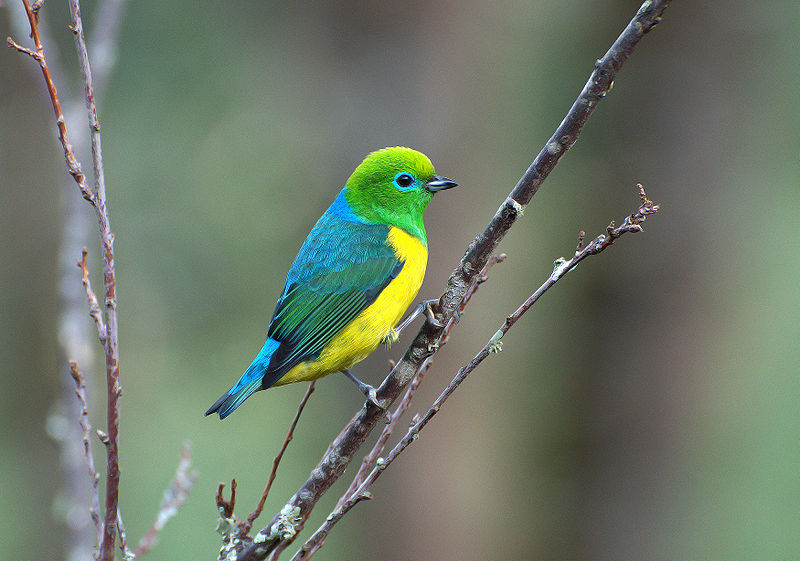
\includegraphics[scale=0.4]{imagens/passaro.jpg}
\end{center}
}
\legend{Fonte: \citeonline{limarka}}
\end{figure}

As imagens são inseridas o mais próximo possível do texto que as
referenciam.

\hypertarget{r}{%
\chapter{R}\label{r}}

\hypertarget{como-inserir-imagens-do-r}{%
\section{Como inserir imagens do R}\label{como-inserir-imagens-do-r}}

A Figura \ref{histograma} é um histograma.

\begin{figure}[htbp]
\hypertarget{histograma}{%
\caption{Exemplo de histograma}\label{histograma}
\begin{center}
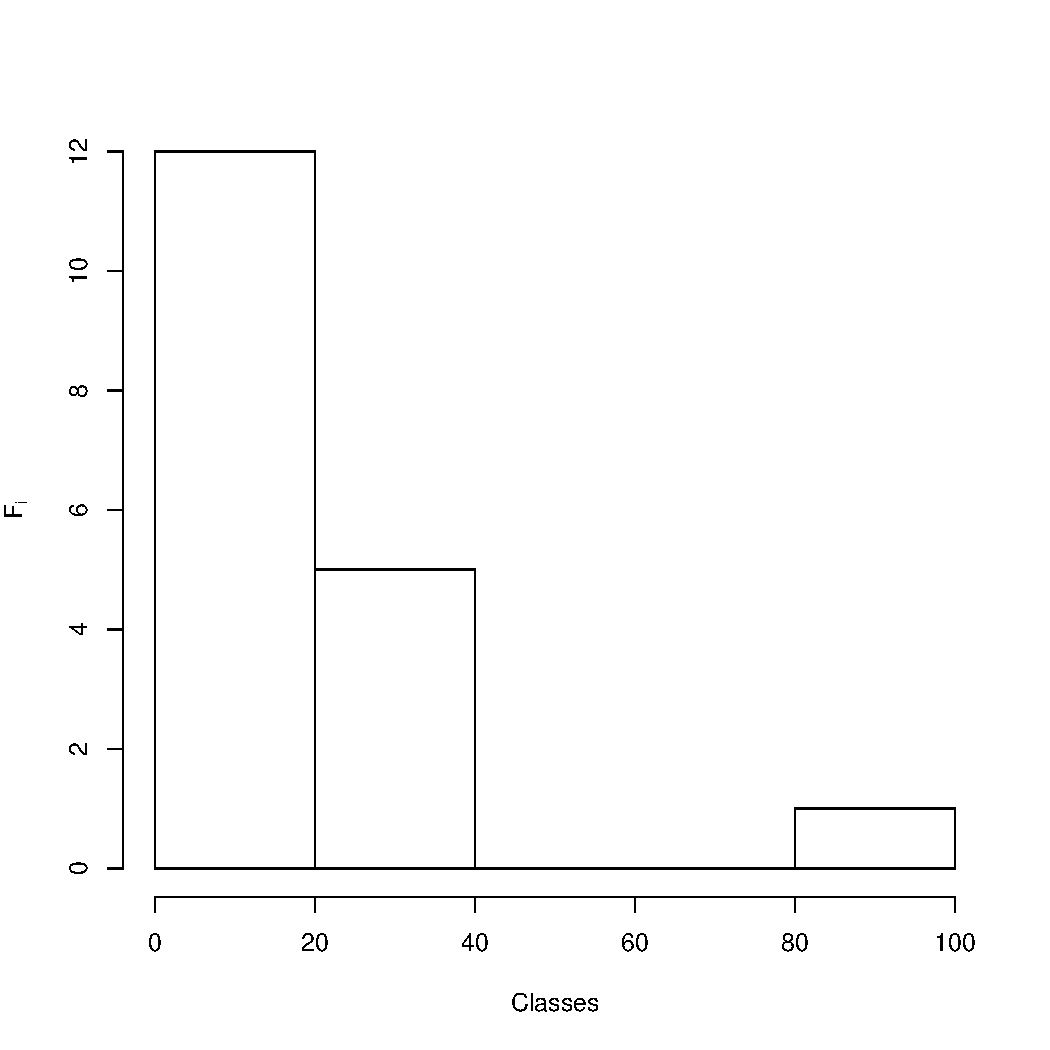
\includegraphics[scale=0.4]{imagens/R/historgrama.pdf}
\end{center}
}
\legend{Fonte: Autor.}
\end{figure}

Para gerar os códigos R, digite \texttt{rake\ r} no terminal. Isso irá
compilar todas os códigos dentro da pasta imagens, com extensão
\texttt{.R} para \texttt{.pdf}, em seguida poderá incluir normalmente
como uma imagem.

\textbf{NOTA}: Certifique-se de ter instalado todos os pacotes R
necessários para compilar sua imagem.

Também é recomendado a utilização do \texttt{guard} para geração
automática quando houver alterações.

\begin{figure}[htbp]
\hypertarget{pizza}{%
\caption{Exemplo de geração de gráfico R}\label{pizza}
\begin{center}
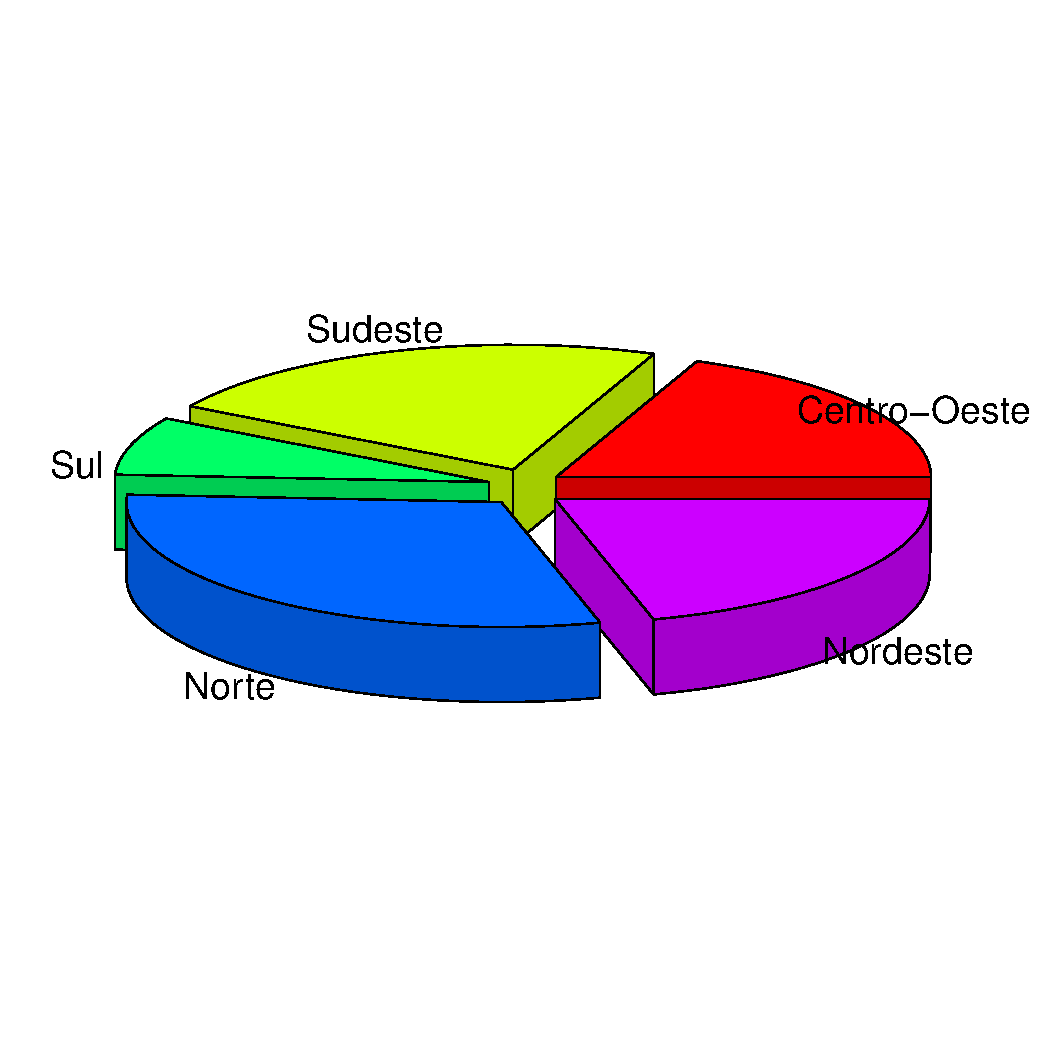
\includegraphics[scale=0.4]{imagens/R/pizza-grafico.pdf}
\end{center}
}
\legend{Fonte: Autor.}
\end{figure}

\hypertarget{dois-gruxe1ficos-r-juntos}{%
\chapter{Dois gráficos R juntos}\label{dois-gruxe1ficos-r-juntos}}

\begin{figure}[htbp]
\hypertarget{doisgraficos}{%
\caption{Exemplo de geração dois gráficos R, lado a lado}\label{doisgraficos}
\begin{center}
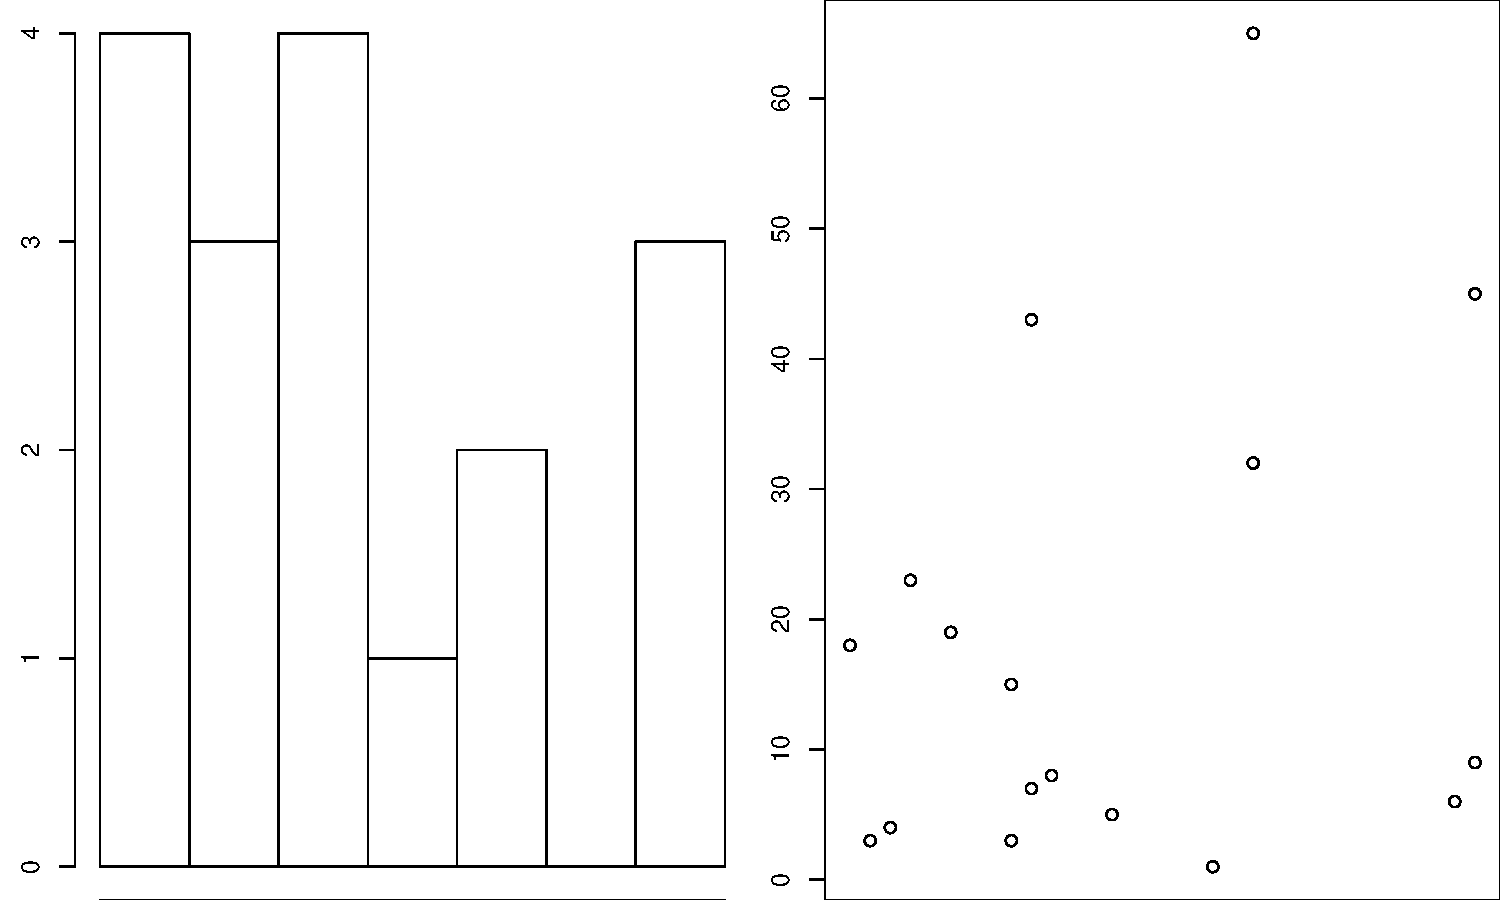
\includegraphics[scale=0.4]{imagens/R/dois-graficos.pdf}
\end{center}
}
\legend{Fonte: Autora.}
\end{figure}

\hypertarget{tabelas}{%
\section{Tabelas}\label{tabelas}}

\begin{longtable}[]{@{}lll@{}}
\caption{Cursos técnicos integrados ao Ensino Médio no IFS \label{tabela_cursos}}\tabularnewline
\toprule
\begin{minipage}[b]{0.13\columnwidth}\raggedright
Curso\strut
\end{minipage} & \begin{minipage}[b]{0.70\columnwidth}\raggedright
Descrição\strut
\end{minipage} & \begin{minipage}[b]{0.08\columnwidth}\raggedright
Duração\strut
\end{minipage}\tabularnewline
\midrule
\endfirsthead
\toprule
\begin{minipage}[b]{0.13\columnwidth}\raggedright
Curso\strut
\end{minipage} & \begin{minipage}[b]{0.70\columnwidth}\raggedright
Descrição\strut
\end{minipage} & \begin{minipage}[b]{0.08\columnwidth}\raggedright
Duração\strut
\end{minipage}\tabularnewline
\midrule
\endhead
\begin{minipage}[t]{0.13\columnwidth}\raggedright
Enfermagem\strut
\end{minipage} & \begin{minipage}[t]{0.70\columnwidth}\raggedright
Capacita o profissional para prestar cuidados de enfermagem.\strut
\end{minipage} & \begin{minipage}[t]{0.08\columnwidth}\raggedright
3 anos\strut
\end{minipage}\tabularnewline
\begin{minipage}[t]{0.13\columnwidth}\raggedright
Informática\strut
\end{minipage} & \begin{minipage}[t]{0.70\columnwidth}\raggedright
Forma o profissional para atuar na instalação, configuração de computadores.\strut
\end{minipage} & \begin{minipage}[t]{0.08\columnwidth}\raggedright
3 anos\strut
\end{minipage}\tabularnewline
\begin{minipage}[t]{0.13\columnwidth}\raggedright
Agropecuária\strut
\end{minipage} & \begin{minipage}[t]{0.70\columnwidth}\raggedright
Habilita o profissional para atuar na gestão de propriedades rurais.\strut
\end{minipage} & \begin{minipage}[t]{0.08\columnwidth}\raggedright
3 anos\strut
\end{minipage}\tabularnewline
\bottomrule
\caption*{Fonte: Autor.}
\end{longtable}

O Instituto Federal de Sergipe (IFS) oferece diversos cursos técnicos
integrados ao ensino médio, que combinam a formação básica com a
profissionalizante. Essa modalidade de ensino é uma excelente opção para
quem deseja se preparar para o mercado de trabalho ou ingressar no
ensino superior.

A \autoref{tabela_cursos} apresenta alguns dos cursos técnicos
integrados ao ensino médio oferecidos pelo IFS, com informações sobre a
descrição do curso, a duração e as habilidades desenvolvidas.

\hypertarget{quadros}{%
\section{Quadros}\label{quadros}}

\renewcommand\LTcaptype{quadro}
\begin{longtable}[]{|c|c|c|c|}
\caption{Perfil dos voluntários do experimento\label{quadro_exemplo}}\tabularnewline
\toprule
Vol. & Formação acadêmica & Experiência c/ Latex & Experiência c/ Markdown\tabularnewline
\midrule
\endhead
1 & Ciência da Computação & ShareLatex & Readme/Github\tabularnewline
2 & Engenharia da Computação & Viu prof. utilizando & -\tabularnewline
3 & Engenheiro elétrico (mestrando) & Utiliza para tudo & -\tabularnewline
\bottomrule
\caption*{Fonte: \citeonline{limarka}}
\end{longtable}
\renewcommand\LTcaptype{table}

O \autoref{quadro_exemplo}, apresenta informações detalhadas sobre os
participantes de um estudo. Ele é um exemplo de como dados podem ser
organizados de forma clara e concisa, facilitando a leitura e a
compreensão.

\hypertarget{expressuxf5es-matemuxe1ticas}{%
\section{Expressões matemáticas}\label{expressuxf5es-matemuxe1ticas}}

Este guia fornece uma introdução rápida à criação de expressões
matemáticas, com exemplos práticos para ilustrar os principais comandos
e recursos.

Exemplos:

\begin{itemize}
\tightlist
\item
  \textbf{Equação do segundo grau}:
  \begin{math} ax^2 + bx + c = 0 \end{math}
\item
  \textbf{Integral definida}:
  \begin{math} \int_a^b f(x) \, dx \end{math}
\end{itemize}

Exemplos de array:

\begin{array}{c|c}
  1 & 2 \\
  \hline
  3 & 4
\end{array}

\hypertarget{citauxe7uxe3o-direta-curta}{%
\section{Citação direta curta}\label{citauxe7uxe3o-direta-curta}}

A expressão `furiosa' dessa estátua de que fala Rabelais, corresponde
também à realidade.'' \cite[p. 5]{abntex2cite}.

\hypertarget{citauxe7uxe3o-direta-longa}{%
\section{Citação direta longa}\label{citauxe7uxe3o-direta-longa}}

\begin{quote}
A `norma' 6023:2000 (2) é complicada e cheia de inconsistências. Jamais
será possível gerar um estilo bibtex totalmente consistente com a
`norma', até porque nem a `norma' é compatível com ela mesma. Um bom
estilo bibliográfico deve ter uma linha lógica para formatação de
referências. Assim, com alguns poucos exemplos, qualquer pessoa poderia
deduzir os casos omissos. Nesse sentido, a `norma' 6023 trafega pela
contra-mão. É quase impossível deduzir sua linha lógica. O problema mais
grave, no entanto, fica pela maneira de organizar nomes. A ABNT quebrou
o sobrenome em duas partes. Normalmente se fala apenas em ``\emph{last
name}'', mas agora temos o ``\emph{last last name}'' graças à ABNT.
\cite[p. 5]{abntex2cite}.
\end{quote}

\hypertarget{citauxe7uxe3o-indireta}{%
\section{Citação indireta}\label{citauxe7uxe3o-indireta}}

A citação indireta é uma forma poderosa para integrar as ideias de
outros autores em seu trabalho de forma criativa e original. Ela permite
que você apresente as ideias e argumentos de outro autor com suas
próprias palavras, seja através de um resumo, tradução ou interpretação.

A citação no texto:

Segundo \citeonline{abntex2cite}, rede de marketing é o resultado do
marketing de relacionamento a partir da construção de um ativo
insubstituível.

O texto original:

\begin{quote}
{[}\ldots{}{]} o resultado do marketing de relacionamento é a construção
de um ativo insubstituível da empresa chamado rede de marketing.
\end{quote}

% ----------------------------------------------------------
% ELEMENTOS PÓS-TEXTUAIS
% ----------------------------------------------------------
\postextual
% ----------------------------------------------------------

% ----------------------------------------------------------
% Início dos ELEMENTOS PÓS-TEXTUAIS
% ----------------------------------------------------------
\postextual
% ----------------------------------------------------------

% ----------------------------------------------------------
% Referências bibliográficas
% ----------------------------------------------------------
\bibliography{xxx-referencias}
% ----------------------------------------------------------
% Apêndices
% ----------------------------------------------------------
%% 
% Seção de apendices configurada como desativada
%% 
% ---

% ----------------------------------------------------------
% Anexos desativados: 
% Seção de anexos configurada como desativada
% ----------------------------------------------------------



\end{document}
